\documentclass[12pt]{article}
\setlength{\topmargin}{-.5in}
\setlength{\textheight}{9in}
\setlength{\oddsidemargin}{.125in}
\setlength{\textwidth}{6.26in}

\usepackage[english]{babel}
\usepackage[utf8]{inputenc}
\usepackage[fleqn]{amsmath}
\usepackage{amssymb}
\usepackage{amsthm}
\usepackage{graphicx}
\usepackage{leftidx}

\usepackage{relsize}
\usepackage{verbatim}
\usepackage{array}
\usepackage{float}
\usepackage{tikz}
\usetikzlibrary{matrix}
\usepackage[all,cmtip]{xy}

\newtheorem{theorem}{Theorem}
\newtheorem{lemma}[theorem]{Lemma}
\newtheorem{proposition}[theorem]{Proposition}
\newtheorem{corollary}[theorem]{Corollary}
\newtheorem{example}[theorem]{Example}

\newenvironment{definition}[1][Definition]{\begin{trivlist}
\item[\hskip \labelsep {\bfseries #1}]}{\end{trivlist}}

\begin{document}

\title{A mathematical approach to analyzing voting power with California as six states}
\author{Steven Nguyen\\
California Lutheran University}
\date{December 11, 2015}
\maketitle
\newpage

\section{Introduction}
A voting system is which voters choose between two alternatives can 
be described as weighted voting system. Weighted voting is sometimes used to vote on candidates but more commonly to decide “yes” or “no” on a proposal. In a weighted voting system, the power of a voter is his or her ability to influence a decision and a group of voters is a winning coalition when the sum of the weights of the voters in the group is greater than or equal to the quota.
One of the most common examples of a voting system is the U.S. Electoral College. Under the Electoral College system, the number of votes for each state is based upon that state's population. California, one of the most populous states, can cast 55 electoral votes while Alaska may cast only 3 votes. In this project we plan to analyze the shift in voting power in the Senate both with the current single California and then with a new six states California using the \textit{Shapley-Shubik power index}. Also, we will examine at how the Electoral College will be affected in both scenarios.    


\subsection{Weighted Voting System}
Suppose five friends are trying to decide whether or not to watch a movie later the evening, and we assume that each friend has one vote. We can describe the situation as a weighted voting system of 5 voters ${\{v_1,v_2,v_3,v_4,v_5\}}$ where each voter has weight 1, since they each have 1 vote and it takes 3 or more votes to win. As seen in \cite{M}, we denote the quota, or number of votes need to win, as q, so here $q=3$ Also, for voter $v_i$ their number of votes or weight is denoted by $w_i$, so $w_i =1$ for each voter. We represent all of this as $$[q:w_1,w_2,w_3,w_4,w_5] = [3:1,1,1,1,1].$$ But what if one friend has three votes since she can get a discount at the movie theater? Then at least 4 votes out of 7 are required to win, and we change the weighted voting system to 


$$[4:3,1,1,1,1]$$ where $v_1$ is the person with the discount. We will specifically take a look at each voters power indices using the \textit{Shapley-Shubik power index} and conclude who is the most influencial voter who turns a losing coalition into a winning coalition most often. Recall from \cite{M}, the following definition of \textit{Shapley-Shubik power index}.
\begin{definition}
\textit{Shapley-Shubik power index} of $v_i$ denoted SSPI($v_i$)

$$SSPI(v_i) = \frac{\text{number of times $v_i$ is pivotal}}{\text{number of voting orders}}$$
\end{definition}
$$ SSPI(v_i) = \frac{\text{number of times $v_i$ pivotal}}{n!}$$
A pivotal voter is the one who joins the prior voters would give the coalition enough votes to win. Thus, we note in each coalition (by underling) the pivotal voter.
\\
\\
\noindent In our previous  example of a weighted voting system $[3:1,1,1,1,1]$, we first list all possible ordering of the five voters ${\{v_1,v_2,v_3,v_4,v_5\}}$ and we start underline the voters from left to right who meet or exceeds the quota. Since with 5 voters there are 5! or 120 possible ways of placement. Although this calculation may seen tedious we can use our understanding of who is a pivotal player in this system. Based on this system $$[3:1,1,1,1,1]$$ we can concluded that spot three is always going to be pivotal because spot three is where we have acquired 3 votes and meet the quota. Since each voter will be in spot 3 there are 24 times where each voter has a Shapley-Shubik power idex of $\frac{24}{120}$ and each voter will have $20\%$ of the voting power.

Another situation we can analyze is when a collection of voters each with weight 1 organize and vote together as a single blocs that is a single voter with a larger weight.
%%%%%%%%%%%%%%%%%%%%%%%%%%%%%%%%%%%%%%%%%%%%%%%%%%%%%%%%%%%%%%%%%%%
\subsubsection{Bloc Voting}
In our previous example, consider this scenario where the 5 friends are trying to decide whether or not to watch a movie during final weeks. Out of the 5 friends: 2 are math majors, 2 are computer science major, and 1 is a business major. Let's assume that the 2 math majors would want vote to stay home. If both the math majors agree to vote the same way as one they can be consider one voter with a voting weight equal to 2. This is an example of bloc voting. A \textit{voting bloc} is a group of voters that agree to all vote the same way together. In forming a bloc, a group acts like a single vote equal to the number of members in the group.
Groups that form a blocs will be denoted with a bar to represent the collective vote while other groups will be assumed to be groups of independent voters with weight one. In this case, the math majors might want to organize as a bloc hoping to wield more influence on the decision. It is important to distinguish who is organizing a bloc because it changes the number of voters in the system. Therefore, a new notation is useful to represent this system.
The \textit{Shapley-Shubik power index} for the single group that forms a bloc is denoted:
\begin{equation}
SSPI(A|\bar{B})
\end{equation}
where $\bar{B}$ is forming a bloc given that $A$ remains independent.
The voting power for a group forming a bloc given there is one other bloc in the voting system is denoted as:\begin{equation}
SSPI(A|\bar{A}\bar{B})
\end{equation}



For this specific example, our new notation, we focus on the groups $$[q:A,B,C] =[3:\bar{2},2,1]$$ where $q= 3$ is our quota and $A=\bar{2}$ represents the math majors voting as a bloc, $B=2$ represents the computer science majors each voting independently and $C=1$ is the single business major.
\\
\\
We can analyze the situation by using the Shapley-Shubik power index when they organized as a bloc. The symbol $[3:\bar{2},2,1]$ represent a body where two math majors formed a bloc in which they are now a group of four voters (call them A,B,C,D) casting 2,1,1,1 votes respectively, and 3 votes are needed to make a decision. We start by figuring out who is the pivotal voter in this scenario and in this system there are 4! possible orderings.
\begin{example}\label{example1}
Calculate the SSPI of B given that $\bar{A}$ is bloc in this weighted voting system $[3:\bar{A},B,C,D]$  
\begin{center}
\begin{tabular}{ l c c r }
  $\bar{A}$ & $\underline{B}$ & $C$ & $D$\\ 
  $\bar{A}$ & $\underline{B}$ & $D$ & $C$\\
  $\bar{A}$ & $\underline{C}$ & $B$ & $D$\\
  $\bar{A}$ & $\underline{C}$ & $D$ & $B$\\
  $\bar{A}$ & $\underline{D}$ & $C$ & $B$\\
  $\bar{A}$ & $\underline{D}$ & $B$ & $D$\\
\end{tabular}
\end{center}
\begin{center}
\begin{tabular}{ l c c r }
  $B$ & $\underline{\bar{A}}$ & $C$ & $D$\\
  $B$ & $\underline{\bar{A}}$ & $D$ & $C$\\
  $B$ & $C$ & $\underline{\bar{A}}$ & $D$\\
  $B$ & $C$ & $\underline{D}$ & $A$\\
  $B$ & $D$ & $\underline{\bar{A}}$ & $C$\\
  $B$ & $D$ & $\underline{C}$ & $\bar{A}$\\
\end{tabular}
\end{center}
\begin{center}
\begin{tabular}{ l c c r }
  $C$ & $\underline{\bar{A}}$ & $B$ & $D$\\
  $C$ & $\underline{\bar{A}}$ & $D$ & $B$\\
  $C$ & $B$ & $\underline{\bar{A}}$ & $D$\\
  $C$ & $B$ & $\underline{D}$ & $\bar{A}$\\
  $C$ & $D$ & $\underline{\bar{A}}$ & $B$\\
  $C$ & $D$ & $\underline{B}$ & $\bar{A}$\\
\end{tabular}
\end{center}
 \begin{center}
\begin{tabular}{ l c c r }
  $D$ & $\underline{\bar{A}}$ & $C$ & $B$\\
  $D$ & $\underline{\bar{A}}$ & $B$ & $C$\\
  $D$ & $C$ & $\underline{\bar{A}}$ & $B$\\
  $D$ & $C$ & $\underline{B}$ & $\bar{A}$\\
  $D$ & $B$ & $\underline{\bar{A}}$ & $C$\\
  $D$ & $B$ & $\underline{C}$ & $\bar{A}$\\
\end{tabular}
\end{center}
\begin{equation}
SSPI(B|\bar{A}) = \frac{4}{24}
\end{equation}
This observation leads us that A has Shapley-Shubik score of $\frac{12}{24}$ and hence A has 50\% of the power while B, C, and D has each 16.7\% of the power. 
\end{example} 
\subsubsection{2 bloc}
When the math majors announced that they are forming a bloc there would be considerable tension that the computer science majors would want to organize too. How does that change the power index?
Our new weighted voting system would be noted as $$[3:\bar{2},\bar{2},1]$$ 
\begin{example}\label{2}
Calculate the SSPI of $A$ and $C$ given that $\bar{A}$ and $\bar{B}$ is bloc in this weighted voting system $[3:\bar{A},B,C]$ 
\begin{center}
\begin{tabular}{ l c r }
  $A$ & $\underline{B}$ & $C$\\ 
  $A$ & $\underline{C}$ & $B$\\
  $B$ & $\underline{A}$ & $C$\\
  $B$ & $\underline{C}$ & $A$\\
  $C$ & $\underline{A}$ & $B$\\
  $C$ & $\underline{B}$ & $A$\\
\end{tabular}
\end{center}
\begin{equation}
SSPI(A|\bar{A}\bar{B}) = \frac{1}{3}
\end{equation}
\begin{equation}
SSPI(C|\bar{A}\bar{B}) = \frac{1}{3}
\end{equation}
Notice that spot two will always pivot 
\end{example}



%%%%%%%%%%%%%%%%%%%%%%%%%%%%%%%%%%%%%%%%%%%%%%%%%%%%%%%%%%%%%%%%%%
\subsubsection{Movement Diagram}
As we have seen the voting influence of a particular group is dependent on their voting weight. When we are dealing with bloc voting we can see the voting power of a group shifts as we change the number of groups that vote as a bloc in the overall system. We can construct a movement diagram to highlight key features in this situation.
\begin{center}
\begin{tabular}{| c | c | c | c |} \hline
         &  &     &           \\
         &  & $B$ & $\overline{B}$ \\ \hline
                &A &.333 &  .500     \\
$A$           &B &.333 &  .250     \\
                &C &.333  & .250     \\ \hline
                &A &.500 &  .333    \\
$\overline{A}$&B &.250 &  .333     \\
                &C &.250 & .333     \\ \hline
\end{tabular}
\end{center}




\section{Six State California}
California is one of the largest states in the U.S. It is third largest in area, but first in terms of population: 38,892,500 (according to the 2014 U.S. Census.) There are many conflicting interests and may feel California has become too large and hard to govern. There have been proposals to split California into six smaller states, one of the more recent being, Tim Draper's proposal to split California into six states. This proposal could be on the 2016 state ballet. Under this proposal, the six new states would be as listed below in the table and shown on the map. We also list population and percentages of Democrats and Republicans in each state. 
\newpage
\begin{figure}
\centering
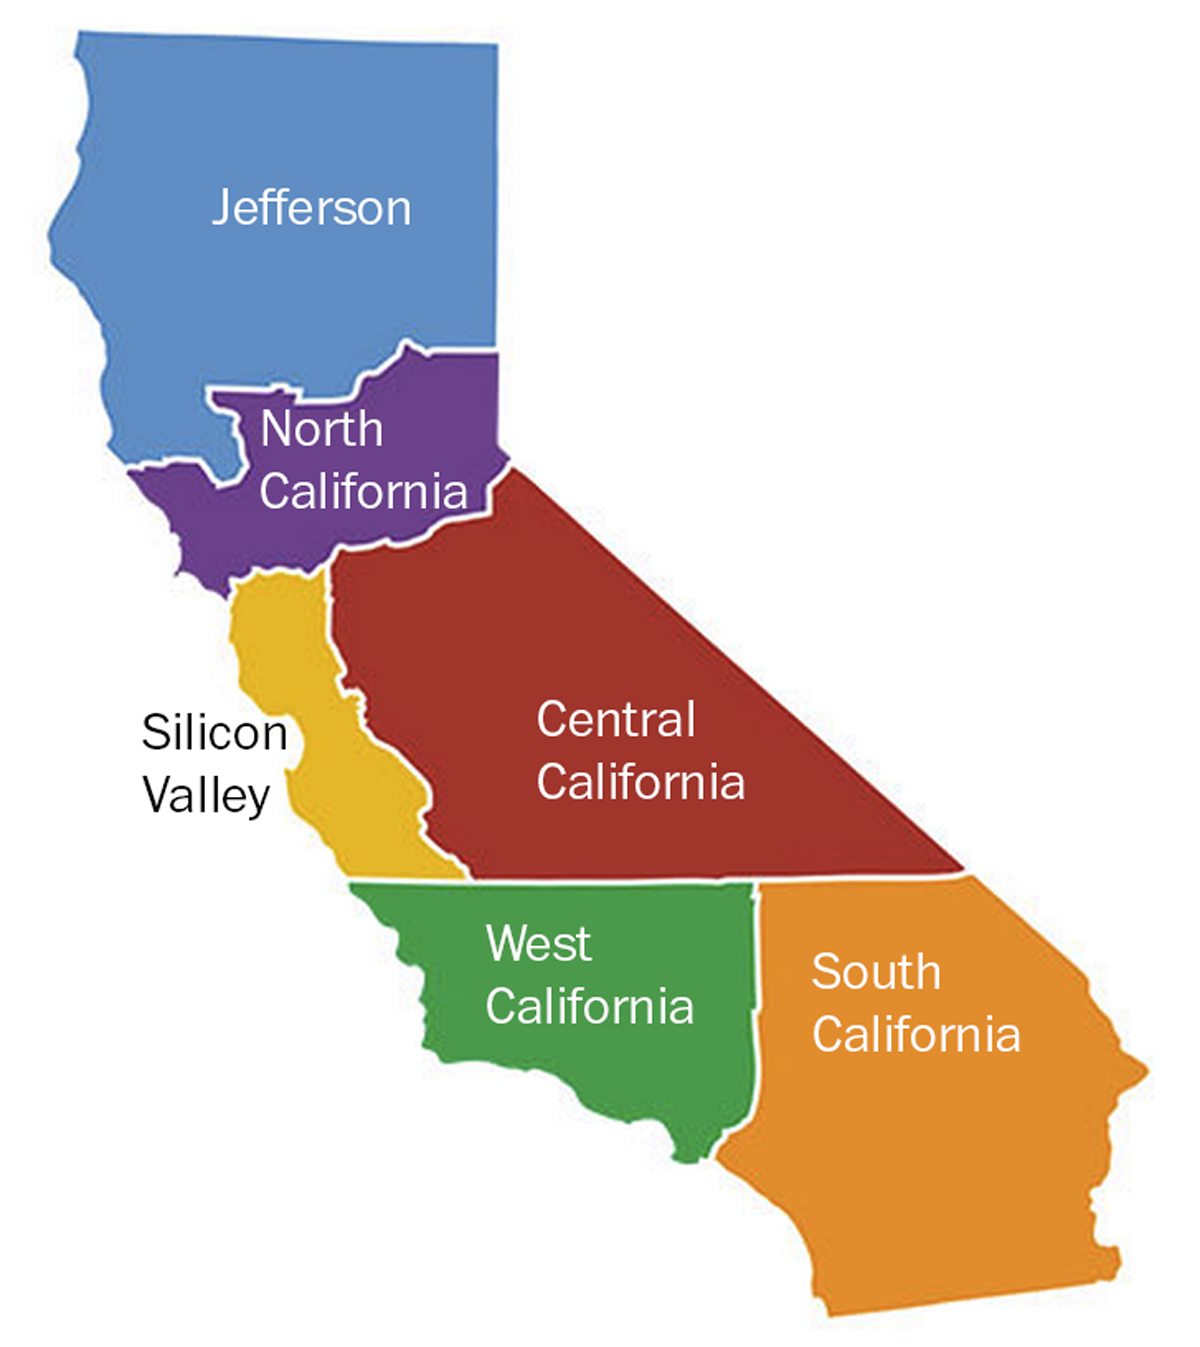
\includegraphics[width=60mm]{six_californias.png}
\caption{Proposed California \label{overflow}}
\end{figure}

\begin{figure}
\begin{center}
\begin{tabular}{ | l | l | l | p{5cm} |}
    \hline
    Six States& Democrats & Republicans \\ \hline
    Jefferson&$36$ & 34 \\ \hline
    North California&$43$ & 38  \\ \hline
    Silicon Valley&$51$ & 18  \\ \hline
    Central California&$39$ & 38 \\ \hline
    West California&$49$ & 23  \\ \hline
    South California&$37$ & 36 \\ \hline
    \end{tabular}
    \caption{Percentage of Democrats \& Republicans \label{overflow}}
\end{center}
\end{figure}

The replacement of California by these six states will change the number of Senators in the U.S. Senate since we need 2 Senators for each state. Thus the number of Senators will increase by 10. The percentage of Democrats versus Republicans in the Senate might also change. In the Electoral College, there will be a change in number of total Electoral College votes. While California has been considered a Democratic state, some of the new state states might not be overly Democratic and will be more like the swing states. We first consider the voting power of a collection of swing states in the Electoral College under both the current Electoral College and the new one if the six states California proposal were to go into effect.


%%%%%%%%%%%%%%%%%%%%%%%%%%%%%%%%%%%%%%%%%%%%%%%%%%%%%
\section{Electoral College}
Presidential election in the United State are generally considered as popular vote contests. Although the majority of people would think that who ever has the most votes will win the election the method of electing a U.S. president is called the Electoral College. The president is elected by a majority of electors apportioned to each state according to its representation in both houses of Congress, as selected (by popular vote), to pledged all of the votes to their the winning candidate in that state. Currently California has the most electors, 55, since the number of electors is the number of the House of Representation and Senators. If California were to split into six states, it would create huge opportunities and risks for both parties in presidential elections. We assume that the vote of all the electors for a state would be based on the political affiliation of the majority of the population.
Based on figure 2, two of the six proposed states: Silicon Valley and West California would be solidly Democratic. Jefferson would tilt towards Republican, and the other three states--- North California, Central California and South California could potentially be Republican or Democratic. 



%%%%%%%%%%%%%%%%%%%%%%%%%%%%%%%%%%%%%%%%%%%%%%%%%%%%%%%%%%%%
\subsection{Swing States}
Recall, the outcome of the 2000 presidential election and it revealed a highly divided political landscape. Former Vice President Al Gore received 50,999,897 popular votes to then-Governor of Texas George W. Bush's 50,456,002 votes. Yet, Gore was not the winner.\cite{C} If California were to split into six states,
George W. Bush would have improve his chances of picking up a state or two presumably North California and South California. We can compute, compare and contrast the power indices of the swing state in ``Power Indices and U.S. Presidental Election" and see how it would change if California is to split into six states. 
\begin{definition} 
A \textit{swing state} is a U.S. state where the two major political parties have similar levels of support among voters, viewed as important in determining the overall result of a presidential election. 
\end{definition}
Using the same the collection of swing states as in \cite{C}. The six swing states with the largest number of electoral voters were Florida (25 electoral votes), Pennysylvania (23), Missouri (11), Tennessee (11), and Washington (11) and Wisconsin (11). We start by calculating the voting power for a system and if we assume that the electoral votes for all but the six most populous swing states split evenly 223-223, we are left with candidates requiring a quota of 47 out of the 92 electoral votes in the swing states. The weighted voting system is denoted as $[47:25,23,11,11,11,11]$ The possible effect of splitting up California is far less clear in presidential elections. The six states would have a total 65 electoral votes. However, we do not plan to compute the system above but we will show an example with the new six state California instead. 

 
\subsection{Swing States within 6 State California}
In addition to the swing states based on \cite{C} what if we were to take out two of the swing states from that article and put in two swing states out of the six California? Note that California is not really a swing state but there is a possibility that one or two might be considered as a swing state. First, we would have to find out the electoral votes for each region. Second, we would go through a computational method to find out the Shapley-Shubik power index. Finally, we would compare the data from our result.
\begin{figure}
\begin{center}
\begin{tabular}{ | l | l | l | p{5cm} |}
    \hline
    Six States& Population & Electoral Votes \\ \hline
    Jefferson&$949\text{k}$ & 3 \\ \hline
    North California&$3.8 \text{mill}$ & 7  \\ \hline
    Silicon Valley&$6.8 \text{mill}$ & 12  \\ \hline
    Central California&$4.2 \text{mill}$ & 8 \\ \hline
    West California&$11.6 \text{mill}$ & 19  \\ \hline
    South California&$10.8 \text{mill}$ & 16 \\ \hline
    \end{tabular}
    \caption{Number of Electoral Votes in a six state California \label{overflow}}
\end{center}
\end{figure}

\noindent Let's consider a simple example to understand this concept. First, we need to define which state are is likely to be considered swing states. Based on population in Figure 3, we have assign the number of electoral votes in each of the six states. Based on the party affiliation in Figure 2, we assume that North California is one of the swing state with 7 electoral votes. For this example, we would pick the three most populous swing states in \cite{C}. Our weighted voting system is now $$[39:25,23,11,11,7]$$ and we represent the five voters using the letters A through E and has a combination of 5!=120. We start by calculating the Shapley-Shubik power index for each swing state. 
Since we do not have the time to find out what are the possible combination for this system we found a better approach by considering the system as who pivots in each spot. In this particular system, the 1st spot has no pivot since no voter in our system does not meet quota. Next, we consider 2nd spot. $$[A B \_ \,\_\, \_] $$ $A's$ weight is 25, but this value does not attain the needed quota of 39 and because voter $B$ votes next, we combine voter $A's$ weight and voter $B's$ weight to meet or exceed the quota. Hence voter $B$ is the pivotal voter. We can rearrange the system as $$[B A \_ \,\_\, \_] $$ and we will still meet the quota but voter $A$ is now the pivotal voter. We go through the possible combination when $A$ or $B$ is in 2nd spot and there are 3! ways for each voter. However, when $C$, $D$, or $E$ is in 2nd spot they do not meet the quota and we go to the next voter in the 3rd spot. For pivot in the 3rd spot we would first consider $A$ or $B$ in the 1st spot and together with two of either $C$, $D$, or $E$. We realized that $A$ or $B$ cannot be in the 2nd spot if $A$ or $B$ is voting in the 1st spot since they will meet the quota. Let's consider $C$ with $A$ or $B$ in the 1st spot and $D$ before $C$. We consider all the possible combination when $C$ is in the 3rd spot with $A$ in the 1st spot and $D$ in the 2nd spot. 
$${AD\,\_ \,BE}$$
$${DA\,\_ \,BE}$$
$${AD\,\_ \,EB}$$
$${DA\,\_ \,EB}$$ 
Thus, we have four combination when $A$ in the 1st spot and $D$ in the 2nd spot. We go through the same method when $A$ in the 1st spot and $E$ in the 2nd spot and when $B$ in the 1st spot and $D$ in the 2nd spot and so forth. We found out that there are 16 ways that $C$ can pivot. Our conclusion is that if $A$ or $B$ is in the 1st spot and $A$ or $B$ cannot be in the 2nd spot, it does not matter who the next voter in the 2nd spot since they will not pivot since they do not meet the quota ($C$ $D$ $E$ cannot pivot in the 2nd spot) therefore the 3rd spot is the next pivotal voter. Therefore, there are a total of 16 ways $C$, $D$, and $E$ can be pivotal. We would consider the scenario if $A$ and $B$ is not in the 1st and 2nd spot. Our conclusion reveals that $\{CDE\}$ never pivot together. Next, we would consider $A$ in the 3rd spot with two groups before it. $$[\_\,\_\,A\,\_\,\_]$$ Since we can choose any group in the 1st spot we have the option of $\dbinom{4}{2}=6$ and in the 2nd spot we have only two options and for the 4th and 5th spot we are left with two choices. Hence, there are 24 options for $A$ to be pivotal. $B$ is also the same structure. We have now exhausted all the possible combination in the 3rd spot and move on to the 4th spot. Let's consider if $A$ or $B$ is in the 4th spot $$\{CDE\}\,\_\,\_$$ Given the fact that we can arrange  $\{CDE\}$ in 3! ways, $A$ or $B$ have a total of six pivotal option each. Finally, we have exhausted all the pivotal spots and have 120 pivots as expected.
$$\text{Total Pivots}: \text{1st spot}+\text{2nd spot}+\text{3rd spot}+\text{4th spot}+\text{5th spot}$$
$$\text{Total Pivots}:0+(6+6)+(24+24+16+16+16)+(6+6)+0 =120$$
\\
\\
\noindent Consider another example where we add another swing state such as South California (16 electoral votes.) How would that change the system? We will use the same approach. 



\begin{example}\label{SSP(CA6)}
The calculated power index for six swing state in the system $[47:25,23,16,7,11,11]$ is
\begin{center}
\begin{tabular}{ | l | l | l | p{5cm} |}
    \hline
    Voter & Number of Pivot & Shapley-Shubik Score \\ \hline
    ${v_1}$ & 216 & $.3$  \\ \hline
    ${v_2}$ & 216 & $.3$ \\ \hline
    ${v_3}$ & 72 & $.1$  \\ \hline
    $v_4$   & 72 & $.1$ \\ \hline
    $v_5$   & 72 & $.1$ \\ \hline
    $v_6$   & 72 & $.1$ \\ \hline
    \end{tabular}
\end{center}
with a total of 720 pivots.
\end{example}

%%%%%%%%%%%%%%%%%%%%%%%%%%%%%%%%%%%%%%%%%%%%%%%%%%%%%%%%%%


\section{Weighted Voting System in the Senate}
There are 100 Senators in the Senate: 54 are Republican, 44 are Democratic, and 2 are Independent. A simple majority of 51 votes will form a winning coalition. We can concluded that the Republicans have 54\% of the votes, Democrats have 44\% of the votes, and the Independents have a merely 2\% of the votes. In a weighted voting system, the power of a voter is his or her ability to influence a decision, a coalition is a set of voters who support a measure is being voted on, and a quota is the minimum number of votes needed to form a winning coalition. Recall that we will use the bar \begin{equation}
SSPI(A|\bar{B})
\end{equation} notation to indicated that each groups that form blocs will represent the collective vote while other groups will be assumed to be groups of independent voters each with weight one. This allowed us to see the division of voters in groups regardless of their decision to vote as a bloc or as independents. For this specific example of the weighted voting system is represented as, $$[q:A,B,C]=[51:54,\bar{44},2].$$
Let's assume that the Democrats will want to bloc vote due to an important bill that will be presented at the Senate. In this case we will represent the voting system as $$[51:54,\bar{44},2]$$ and it will have 57 voters, 54 Republicans, 2 Independents, and 1 Democrats of weight 44. 
\\
\\
\noindent We can analyze this situation by using the Shapley-Shubik power index to calculate the total power of the Democrat's power. The most important voter (the pivotal voter) is the one who turns a losing coalition into a winning coalition. Since 51 voters are needed to pass a bill. In order to calculate the Shapley-Shubik power index for the Democrats we will break it into two cases: where the Republicans is placed before the Democrats, and where the Republicans is placed after. First, consider where the Republicans is placed before the Democrats. Originally, the pivot point is placed where we break the quota at 51. With the Democrats placed prior, The last pivot position is moved to $q-w_1+1$ In this situation, the first pivot position would be the eighth place, immediately after the Republicans. 
\begin{center}
\begin{tabular}{ | l | l | l | p{5cm} |}
    \hline
    Democrat Pivot Position & Position for Republican \\ \hline
    $8$ & 7 \\ \hline
    $9$ & 8  \\ \hline
    $10$ & 9  \\ \hline
    $11$ & 10 \\ \hline
    $12$ & 11  \\ \hline
    $13$ & 12  \\ \hline
    $14$ & 13 \\ \hline
    $15$ & 14  \\ \hline
    $\vdots$&\vdots \\ \hline
    $51$ & 44  \\ \hline
    \end{tabular}
\end{center}
We can take the 44 cases and calculate the possible combinations where the Democrats is in a pivotal position given that the Republicans is placed first to be:


$$SSPI(D) = \frac{44 * 56!}{57!} = \frac{44}{57}$$

\noindent A careful inspection reveals that if the Democrats organized, there total power will increased from 44\% to 77.2\%. The Democrats will pivot if it joins a coalition between 8 through 51. In order words, the Democrats will have $\frac{44}{57}$ or 77.2 percent of the power. The Republicans who just had 54 percent of the total power before the Democrats bloc vote will now have 23 percent of the power.
\\
\\
In all fairness, if the Democrats organized as a bloc then there will be a high chance that the Republicans will want to organized as a bloc too. If that happened, we would have a game of 4 voters: 2 casting as a single vote, the Republicans casting 54, and the Democrats casting 44.
$$[q:A,B,C]=[51: \bar{54},\bar{44},2]$$
However, this result is very easy to conclude since the Democrats and the Independents could never have enough votes to reach the quota, therefore, the Republicans will always pivot. A careful inspection reveals that when we complete the Shapley-Shubpik power index for the Republicans they will always be pivotal. In other words, the Democrats and the Independents will have no voting power. However, when the Republicans form a bloc the weight exceeds the quota and in fact, the Republicans can pass any measure.  A voter who has no voting power is called a \textit{dummy voter}. In $[51: \bar{54},\bar{44},2]$, the Republicans with weight 54 is called the \textit{dictator} because it is impossible for the Democrats and the Independents  to have a voting power when the Republicans form a bloc. 
\begin{example}\label{example3}
The Shapley-Shubik Power Index for Republicans,Democrats,and Independent when the Republican are bloc
\begin{equation}
SSPI(A|\bar{A}\bar{B}) = 1
\end{equation}
\begin{equation}
SSPI(B|\bar{A}\bar{B}) = 0
\end{equation}
\begin{equation}
SSPI(C|\bar{A}\bar{B}) = 0
\end{equation}
\end{example}



\subsection{Additional Senators in Six State California}
Recall, in our last paper that the number of U.S. Senators would increase by 10 Senators since each state is required to have two Senators.\cite{T} We have concluded based on party affiliation in each new state that four Republicans and six Democrats are added to the six state California. That will bring us a total of 110 Senators. Now, how does that affect the voting power when the additional Senators are added? The new weighted voting system is $$[56:58,50,2]$$


\subsection{Blocs with Republicans splitting into 2 groups}
Although the Tea party is more prominent in the House, we consider the possible situation where the 54 Republicans have subset from the Tea party. What if the Republicans keep the same number of seats but 10 of them formed their own blocs? We start with calculating the power of an organized bloc with an additional group that organized as a bloc. In this example, $$[56:\bar{50}, 48,\bar{10},2]$$
where $q= 56$ is our quota and $A=\bar{50}$ represents the Democrats, $B=48$ represents the Republicans each voting independently and $C=\bar{10}$ represents the Tea party, and $D=2$ represents the Independents. 
we will evaluate the situation where our additional bloc is placed prior. There are two cases: the first where the bloc we are not calculating the power of is placed before the pivot position, and the second where the bloc is placed after.

\begin{example}\label{SSP(CA6)}
Calculate the Shapley-Shubik Power for $\bar{A}$ with Republicans splitting into 2 groups given that $\bar{C}$.
$$[56:\bar{50}, 48,\bar{10},2]$$
\begin{equation}
SSPI(\bar{A}) = \text{two cases with two blocs}
\end{equation}
\begin{equation}
SSPI(\bar{A})=\frac{\text{Case 1}+\text{Case 2}}{52!}
\end{equation}
Case 1: $[\_ \, \bar{A},\bar{C}]$
Where we put the Tea party after the Democrats.
Case 2: $[\bar{C},\bar{A},\_]$
Where we put the Tea party before the Democrats. 
\begin{equation}
Case\,1=[\_ \, \bar{A},\bar{C}]
\end{equation}
We can place $\bar{A}$ is in the 7th spot. With $\bar{C}$ voting after $\bar{A}$, the original pivot position has shifted to $[v-(q-b)+1]=[52-(56-50)+1]$ from spot 45.  $\bar{A}$ can pivot in this position, or even closer to the front while still remaining pivotal. The pivotal spots for $\bar{A}$ are $[7,8,...51]$ and we can reduce the system to $[1,2...45].$ Then we fill in the rest of spots $50!$
We can use summation to sum up the pivotal spots for $\bar{A}$
$${\sum\limits_{i=1}^{45}=45(\frac{45+1}{2})} = 1035.$$
Now, we focus our attention on case 2.
\begin{equation}
Case\, 2=[\bar{C},\bar{A},\_]
\end{equation}
With $\bar{C}$ in front, the earliest pivot position has shifted to the 2nd spot. $\bar{A}$ can pivot from spot $[2...47]$ Again, we use the same technique as above. 
$${\sum\limits_{i=1}^{46}=46(\frac{46+1}{2})} = 1081.$$
\begin{equation}
SSPI(\bar{A})=50!\frac{\text{Case 1}+\text{Case 2}}{52!}=\frac{1035+1081}{52*51} = 79.8\%
\end{equation}
Note that we can use the same approach to calculate the $SSPI(\bar{C}).$
\end{example}
Calculating the power of an independent voter in a system with two groups of voters forming blocs starts to become difficult. 
\begin{example}
Calculate the Shapley-Shubik Power Index for B given that $\bar{A}$ and $\bar{C}$ is bloc
\begin{equation}
SSPI(B|\bar{A}\bar{C})
\end{equation}
We break this down into 4 separate cases. 
Case 1: $[\bar{A}\bar{C},B,\_]$
Where we put the Democrats and Tea party before the Democrats.
Case 2: $[\bar{C},B,\bar{A}]$
Where we put the Republicans between the Tea party and the Democrats. 
Case 3: $[\bar{A} \, B,\bar{C}]$
Where we put the Republicans between the Democrats and the Tea party.
Case 4: $[\_ \,B,\bar{A}\bar{C}]$
Where we put the Tea party and the Democrats after the Republicans.
\\
\\
\par Notice that $B$ cannot pivot in case 1 since $\bar{A}$ and $\bar{C}$ will exceed the quota. Also, $B$ cannot pivot in case 2 since there is not enough votes. Therefore, we simplify our cases to case 2 and 3. The following method is used as above. 
\end{example}

%%%%%%%%%%%%%%%%%%%%%%%%%%%%%%%%%%%%%%%%%%%%%%%%%%%%%%%%%%%%%%%%%
\subsection{Movement Diagram}
Now that we have calculated the power indices for the current California and the six states California, we can conduct a movement diagram to show our results. Below is a table of results for the current California versus the six state California

\begin{figure}
\begin{center}
\begin{tabular}{| c | c | c | c |} \hline
         &  &     &           \\
         &  & $R$ & $\overline{R}$ \\ \hline
                &D &.44 &  0     \\
$D$           &R &.54 &  1     \\
                &I &.02  & 0      \\ \hline
                &D &.7719 &  0    \\
$\overline{D}$&R &.2199 &  1     \\
                &I &.0082 & 0     \\ \hline
\end{tabular}
    \caption{Current California \label{overflow}}
\end{center}
\end{figure}

 \begin{center}
\begin{tabular}{| c | c | c | c |} \hline
         &  &     &           \\
         &  & $R$ & $\overline{R}$ \\ \hline
                &D &.455 &  0     \\
$D$           &R &.527 &  1     \\
                &I &.018  & 0      \\ \hline
                &D &.819 &  0    \\
$\overline{D}$&R &.174 &  1     \\
                &I &.007 & 0     \\ \hline
\end{tabular}
\end{center}

\begin{figure}
\begin{center}
\begin{tabular}{| c | c | c | c |} \hline
         &  &     &           \\
         &  & $R$ & $\overline{R}$ \\ \hline
                &D &.44 &  0     \\
$D$           &R &.54 &  1     \\
                &I &.02  & 0      \\ \hline
                &D &.7719 &  0    \\
$\overline{D}$&R &.2199 &  1     \\
                &I &.0082 & 0     \\ \hline
\end{tabular}
    \caption{Current California \label{overflow}}
\end{center}
\end{figure}
\begin{figure}
\begin{center}
\begin{tabular}{| c | c | c | c |} \hline
         &  &     &           \\
         &  & $R$ & $\overline{R}$ \\ \hline
                &D &.455 &  0     \\
$D$           &R &.527 &  1     \\
                &I &.018  & 0      \\ \hline
                &D &.819 &  0    \\
$\overline{D}$&R &.174 &  1     \\
                &I &.007 & 0     \\ \hline
\end{tabular}
    \caption{Six State California \label{overflow}}
\end{center}
\end{figure}

\newpage Recall from our background paper that the direction of the movement diagram is determine by the direction has a greater power increase. Below is a diagram for our system:

\begin{displaymath}
 \xymatrix{ D,R \ar[r]  \ar[d]
 & D,\overline{R} \ar[d] \\
 \overline{D},R \ar[r] &  \overline{D},\overline{R} }
\end{displaymath}
Note that $\bar{D}$ and $\bar{R}$ has a stable point when they are both bloc. However, we concluded that $\bar{D}$ and $\bar{R}$ should not bloc because does not offer the best voting power for the two groups. 
\section{Conclusion}
Through the use of the Shapley-Shubik Power Index and Movement Diagram we were able to analyze the voting system in the Electoral College and the Senate with the current California and the six state California. In the Electoral College, presidential candidates can greatly appreciate the new swing states in the six state California. These states would received much more attention from the candidates and the voters. In the Senate, the Democrats would not benefit from organizing as a bloc since it is likely that the Republicans will want to organize as a bloc too. In addition to the 10 Senators in the six state California the voting power did not change since the Republicans still had a greater voting power. However, when we describe the situation when the Republicans were splitting into 2 groups the Democrats voting power slightly increase. 

\begin{thebibliography}{10}
\bibitem{C} Colen S. Yong, Channa Navarna, Jung Colen and Jinho Kim, ``Power Indices and U.S. Presidential Elections,'' \emph{The Mathematics Teacher} Vol. 106, pp. 184-190.
\bibitem{F} Fogel, Karrolyne, Kay Somers, Angela Spalsbury, Jennifer Wilson, ``Geometry of Power Indices," \emph{DIMACS Center for Discrete Mathematics and Theoretical Computer Science}, Module 09-1, August 2008.
\bibitem{M} Jeska, Devyn, Steven Nguyen, "New to the Bloc: Mathematics Behind Weighted Voting Systems," California Lutheran University Preliminary Report, October 2015.
\bibitem{J} Jones, Michael D., ``The Geometry behind Paradoxes of Voting Power,'' \emph{Mathematics Magazine}, pp. 103-116, April 2009.
\bibitem{N} Newville, Jessica, ``Voting Theory," Presentation Slides. California Lutheran University, May 2008.
\bibitem{T} Nguyen, Steven, ``Project Proposal: A mathematical approach to analzying voting power with California as six states.'' California Lutheran University, May 2015.
\bibitem{S} Straffin Jr., Philip D., ``The Power of Voting Blocs: An Example," \emph{Mathematics Magazine}, pp.22-24, Jan 1977.
\bibitem{S} Straffin Jr., Philip D., ``Game Theory and Strategy" \emph{The Mathematical Association of America}, pp.3-12, Jan 1993.
\end{thebibliography}



\end{document}

